\documentclass[10pt,a4paper]{article}
\usepackage[margin=0.55in]{geometry}
\usepackage[T1]{fontenc}
\usepackage{lmodern}
\usepackage{xcolor}
\usepackage{graphicx}
\usepackage{booktabs}
\usepackage{tabularx}
\usepackage{enumitem}
\usepackage{titlesec}
\usepackage{fancyhdr}

% High-contrast institutional palette (zero emojis)
\definecolor{navy}{HTML}{1B365D}
\definecolor{crimson}{HTML}{B91C1C}
\definecolor{slate}{HTML}{334155}
\definecolor{lightgray}{HTML}{F1F5F9}
\definecolor{bordergray}{HTML}{CBD5E1}

\pagestyle{fancy}
\fancyhf{}
\renewcommand{\headrulewidth}{0pt}
\fancyfoot[C]{\scriptsize\color{slate} Bengaluru Urban Services \& Mobility Cell \quad|\quad Data Window: Nov 2025 – Nov 2026 ($N = 226,171$ Validated Records) \quad|\quad Page 1 of 1}

\titleformat{\section}{\large\bfseries\color{navy}}{}{0em}{}[\vspace{-6pt}\rule{\textwidth}{0.8pt}]
\titlespacing*{\section}{0pt}{8pt}{5pt}

\setlength{\parindent}{0pt}
\setlength{\parskip}{3.5pt}

\begin{document}

% --- TOP HEADER BANNER ---
\noindent\fcolorbox{navy}{navy}{%
\begin{minipage}{\dimexpr\textwidth-2\fboxsep-2\fboxrule\relax}
    \vspace{4pt}
    {\Large\bfseries\color{white} OPERATIONAL DECISION BRIEF: THE 8 PM AIR QUALITY SURGE}\\[2pt]
    {\small\color{lightgray} Actionable Corridor Triage, Weather Triggers \& Holiday Exodus Protocols for Bengaluru}
    \vspace{4pt}
\end{minipage}}

\vspace{5pt}

% --- MEMO METADATA BLOCK ---
\noindent\fcolorbox{bordergray}{lightgray}{%
\begin{minipage}{\dimexpr\textwidth-2\fboxsep-2\fboxrule\relax}
\small
\begin{tabularx}{\textwidth}{@{}l X l X@{}}
\textbf{\color{navy}TO:} & Office of the Commissioner \& Urban Services Cell & \textbf{\color{navy}DATE:} & November 26, 2026 \\
\textbf{\color{navy}FROM:} & Chandan K S, Data Analytics & \textbf{\color{navy}WINDOW:} & 19:00 – 21:00 IST (Daily Peak) \\
\end{tabularx}
\end{minipage}}

\section{Executive Situation Assessment}
Between \textbf{19:00 and 21:00 IST ("The 8 PM Problem")}, Bengaluru experiences a consistent citywide spike in fine particulate matter ($\text{PM}_{2.5}$), rising \textbf{+23.8\%} over afternoon levels (\textbf{32.30 vs. 26.10 $\mu\text{g/m}^3$}). Cross-referencing 10 CPCB/KSPCB stations with hourly meteorology and Karnataka holiday calendars identifies three operational realities that overturn conventional deployment assumptions:

\begin{itemize}[leftmargin=1.4em, itemsep=1.5pt, topsep=2pt]
    \item \textbf{Corridor-Specific Bottlenecks:} Evening congestion surges at commuter hubs---\textbf{Hebbal (+9.39 $\mu\text{g/m}^3$)} and \textbf{Silk Board (+8.99 $\mu\text{g/m}^3$)}---whereas industrial \textbf{Peenya (-0.67 $\mu\text{g/m}^3$)} drops in the evening.
    \item \textbf{The Rain Washout Paradox:} Rain causes traffic delays, yet cuts 8 PM $\text{PM}_{2.5}$ in half (\textbf{19.50 vs. 39.92 $\mu\text{g/m}^3$} on dry nights; \textbf{-51.2\%}). \textbf{Dry, low-wind evenings ($<8\text{ km/h}$)} are the true respiratory hazard.
    \item \textbf{7-Day Persistence \& Exodus Spikes:} Weekend 8 PM pollution (\textbf{32.50 $\mu\text{g/m}^3$}) equals Tue--Thu office nights, while \textbf{Pre-Long-Weekend / Festival Exodus Evenings} spike an additional \textbf{+25.8\%} (\textbf{38.50 vs. 30.60 $\mu\text{g/m}^3$}).
\end{itemize}

\section{Visual Evidence: Corridor Hotspots \& Rain Scavenging}
\begin{center}
\begin{minipage}{0.49\textwidth}
    \centering
    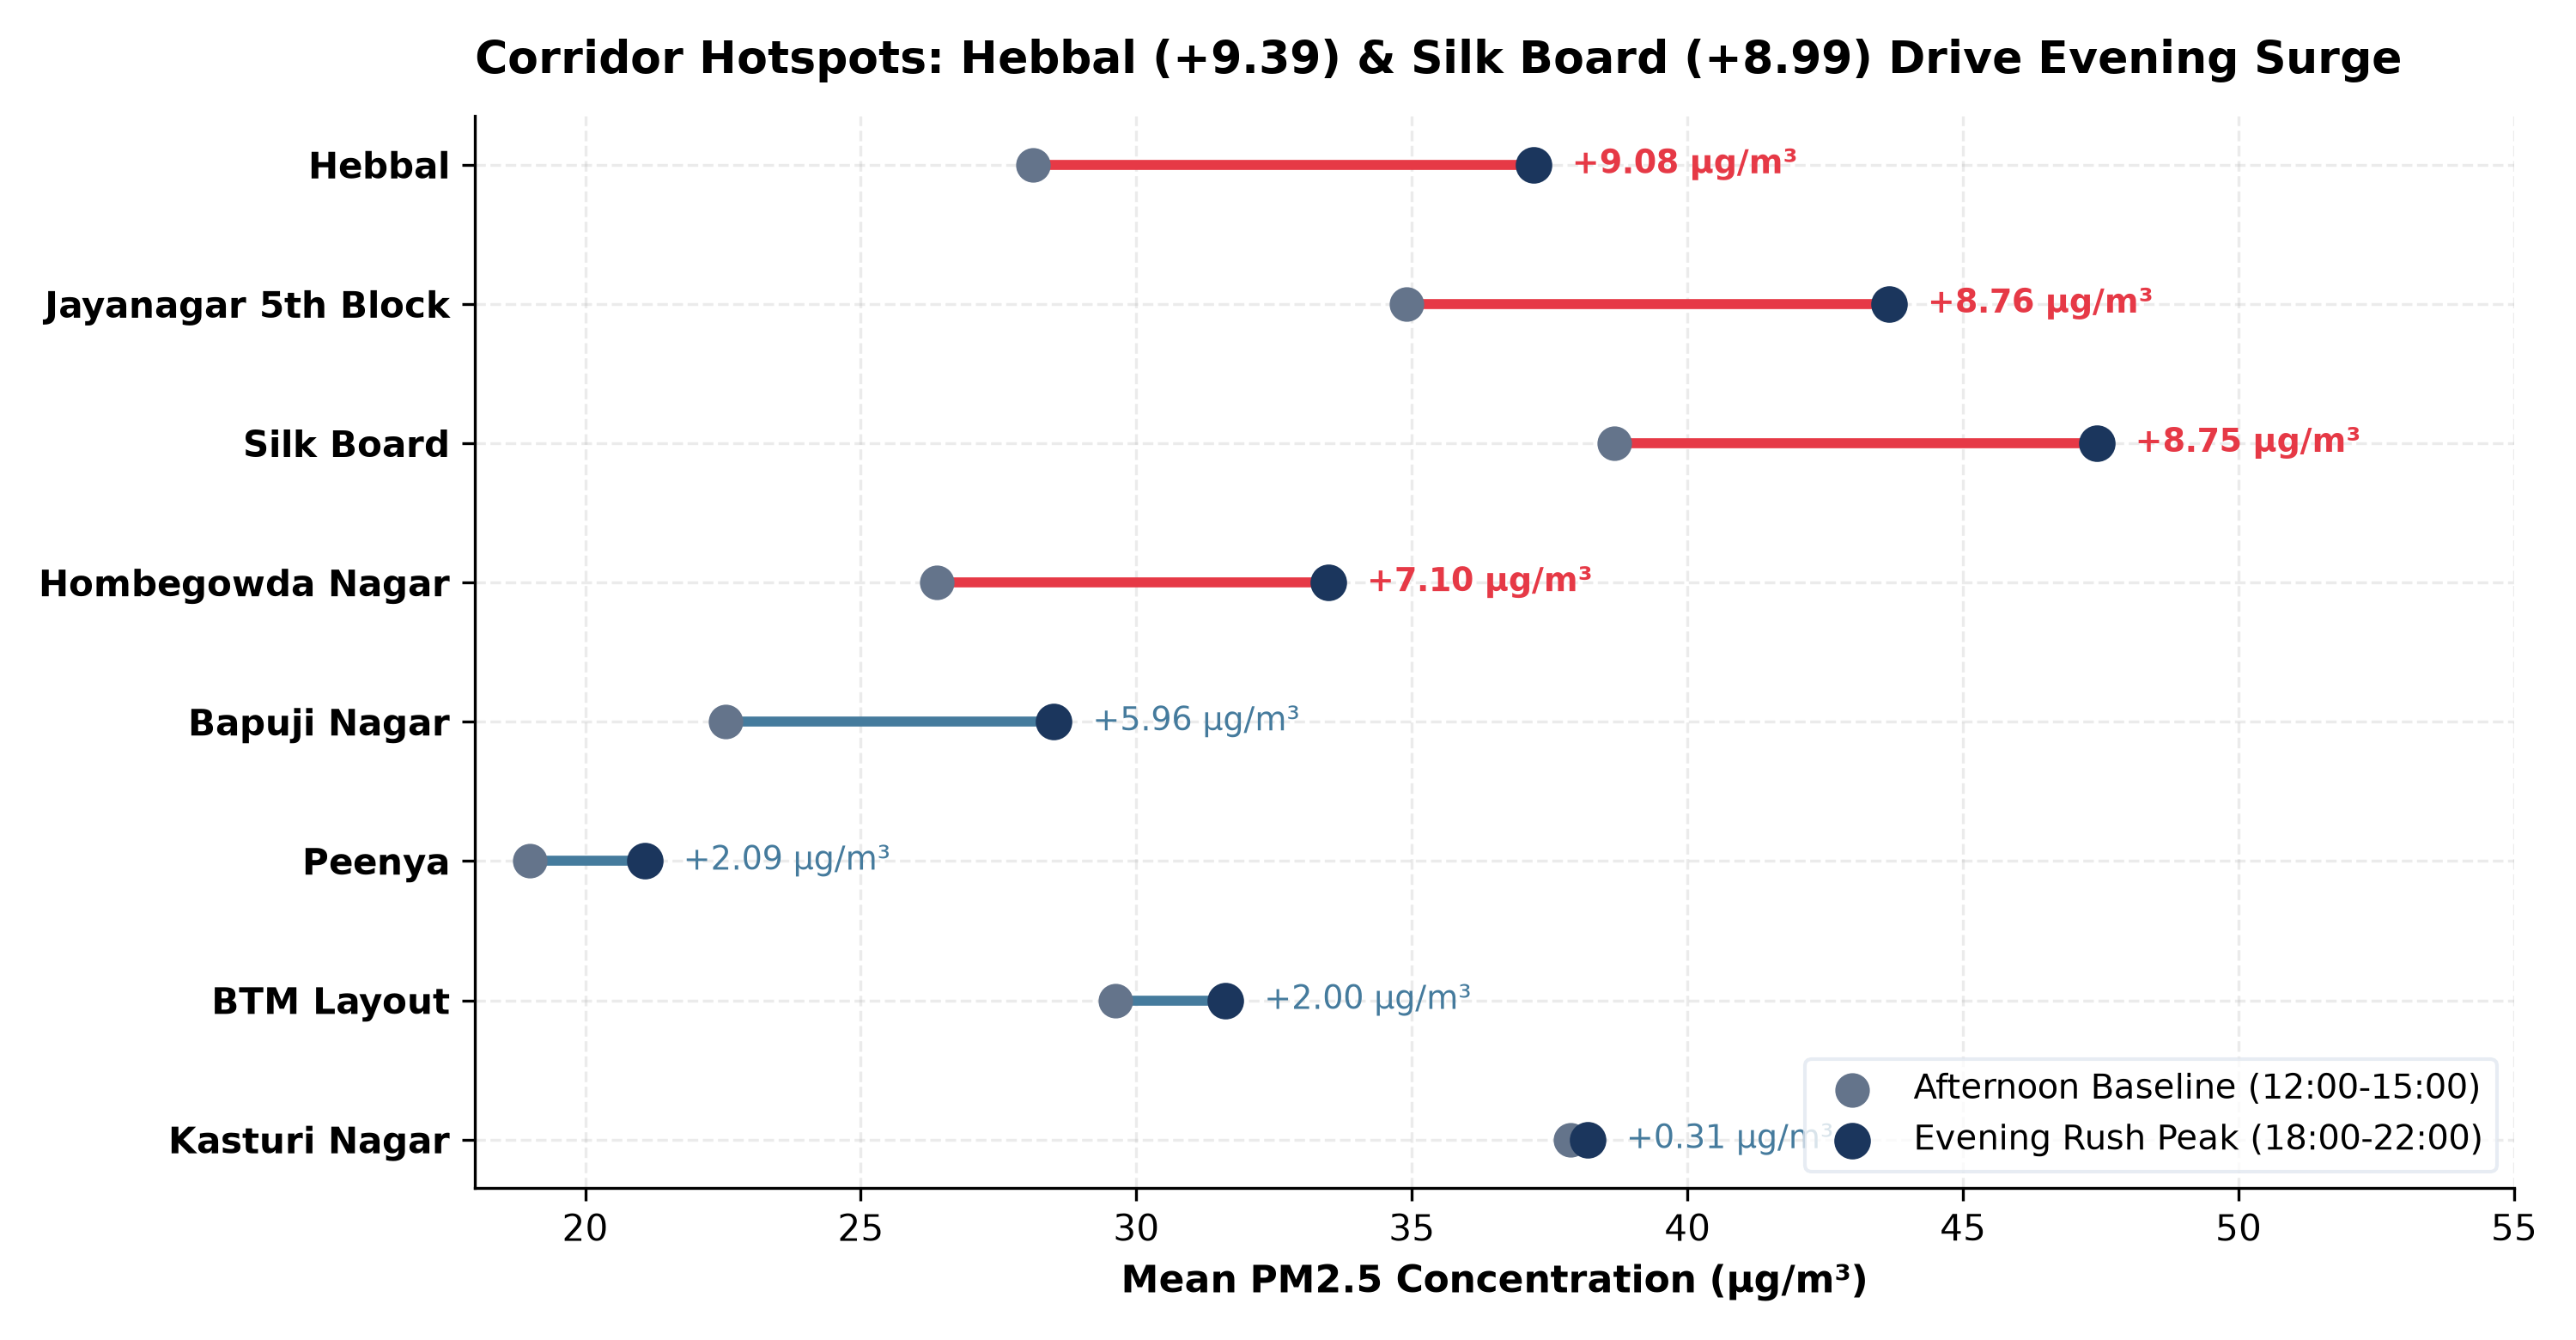
\includegraphics[width=\linewidth]{../outputs/fig2_corridor_surge_dumbbell.png}
\end{minipage}\hfill
\begin{minipage}{0.49\textwidth}
    \centering
    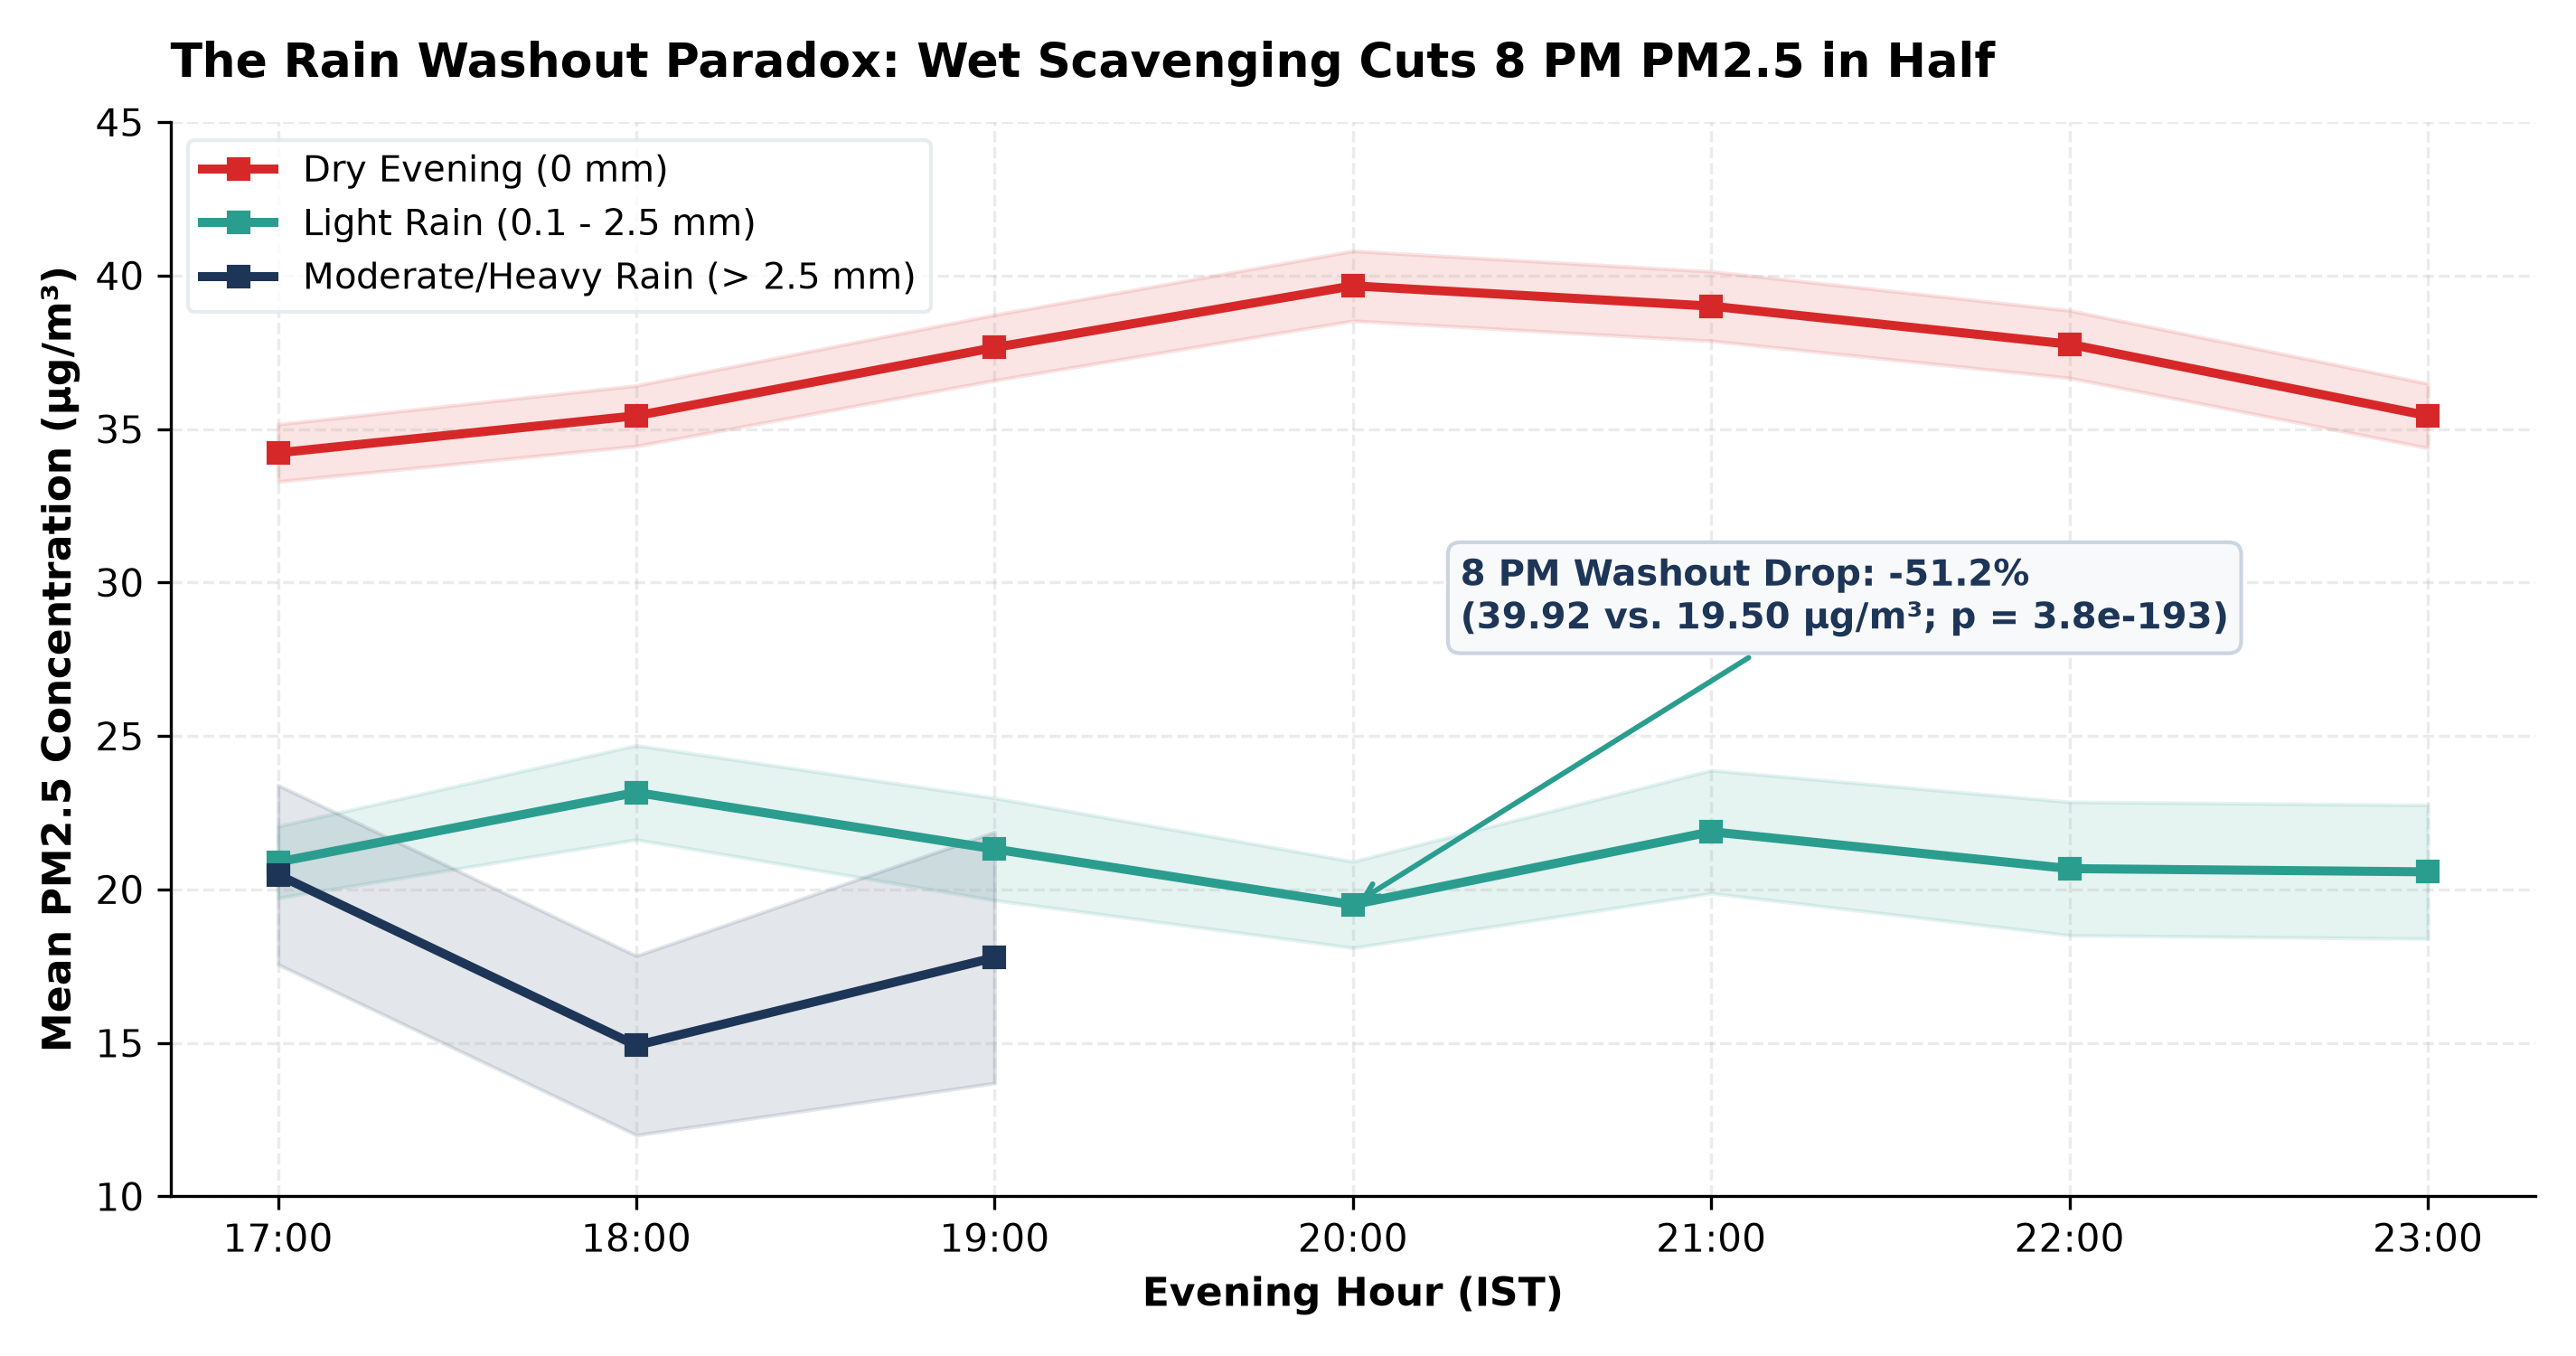
\includegraphics[width=\linewidth]{../outputs/fig3_rain_washout_paradox.png}
\end{minipage}
\end{center}

\section{Recommended Command Decisions \& Deployment Matrix}
\renewcommand{\arraystretch}{1.22}
\small
\begin{tabularx}{\textwidth}{@{}p{3.4cm} p{3.5cm} X@{}}
\toprule
\textbf{\color{navy}Operational Trigger} & \textbf{\color{navy}Target Corridors} & \textbf{\color{navy}Immediate Field Action} \\
\midrule
\textbf{1. Daily 8 PM Window} \newline (18:00--21:30 IST, \textbf{All 7 Days}) & Hebbal Flyover (+9.39), Silk Board (+8.99), Jayanagar (+8.76) & Deploy adaptive traffic signal green-waves and strict BMTC bus-lane enforcement across all 7 days; reallocate evening pollution patrols away from Peenya. \\
\textbf{2. Dry \& Calm Evenings} \newline (Rain = 0 mm, Wind $< 8\text{ km/h}$) & Outer Ring Road, Bellary Rd (NH-44), Hosur Rd (NH-48) & Issue automated health advisories for outdoor traffic personnel and trigger BBMP mechanical road misting (rainy evenings self-clean by -51.2\%). \\
\textbf{3. Pre-Holiday Exodus} \newline (16:00--22:00 IST before long weekends) & Hebbal Exit (NH-44), Silk Board / Electronic City (NH-48) & Pre-activate staggered heavy-freight bans 24 hours ahead and increase Metro/BMTC feeder frequency to curb the +25.8\% exodus surge. \\
\bottomrule
\end{tabularx}

\end{document}
